\documentclass{article}
\usepackage{bm}
\usepackage{amsmath}
\usepackage{graphicx}
\usepackage{mdwlist}
\usepackage[colorlinks=true]{hyperref}
\usepackage{geometry}
\geometry{margin=1in}
\geometry{headheight=2in}
\geometry{top=2in}
\usepackage{palatino}
%\renewcommand{\rmdefault}{palatino}
\usepackage{fancyhdr}
%\pagestyle{fancy}
\rhead{}
\lhead{}
\chead{%
  {\vbox{%
      \vspace{2mm}
      \large
      Introduction to Deep Learning M2177.0043 \hfill
\\
      Seoul National University
      \\[4mm]
      Homework \#\textbf{1}\\
      \textbf{Donghak Lee}
    }
  }
}


\usepackage{paralist}

\usepackage{todonotes}
\setlength{\marginparwidth}{2.15cm}

\usepackage{tikz}
\usetikzlibrary{positioning,shapes,backgrounds}

\begin{document}
\pagestyle{fancy}

\section*{INSTRUCTIONS}

\begin{itemize*}
\item Anything
  that is received after the deadline will be considered to be late and we do not receive late homeworks. We do however ignore your lowest homework grade. 
\item Answers to every theory questions need to be submitted
  electronically on ETL. Only PDF generated from LaTex is accepted.
\item Make sure you prepare the answers to each question
  separately. This helps us dispatch the problems to different graders.
\item Collaboration on solving the homework is allowed. Discussions
  are encouraged but you should think about the problems on your own. 
\item If you do collaborate with someone or use a book or website, you
  are expected to write up your solution independently.  That is,
  close the book and all of your notes before starting to write up
  your solution. 
\end{itemize*}

%!TEX root = hw1_2017-12751.tex

%% Q1
\section{Learning LaTex}

\subsection {}
\begin{center}
\begin{tabular}{|c|c|}
\hline
Donghak & Lee \\
\hline
Computer Science and Engineering & 2017-12751 \\
\hline
\end{tabular}
\end{center}

\subsection {}
\begin{center}
\includegraphics{동학증명사진.jpg}
\end{center}
	
%% Q2
\section{Inverse transform sampling}

\subsection {Probability integral transform}

By properties of pdf, $F_X(x)$ is invertible function with range (0, 1). 
So $\forall y \in (0, 1)$, \[F_Y(y) = P(Y \leq y) = P(F_X(X) \leq y) = P(X \leq F_X^{-1}(y)) = F_X(F_X^{-1}(y)) = y\]
\[f_Y(y) = F_Y'(y) = 1\]
Therefore, random variable Y is uniformly distributed in [0, 1].

\subsection {Inverse transform sampling}

Because random variable U is uniformly distributed in [0, 1], pdf $f_U(u) = 1$. So,
\[P(F_X^{-1}(U) \leq x) = P(F_X(F_X^{-1}(U)) \leq F_X(x)) = P(U \leq F_X(x)) = F_X(x)\]
Therefore, cdf of $F_X^{-1}(U)$ is $F_X(x)$

\subsection {}
\begin{center}
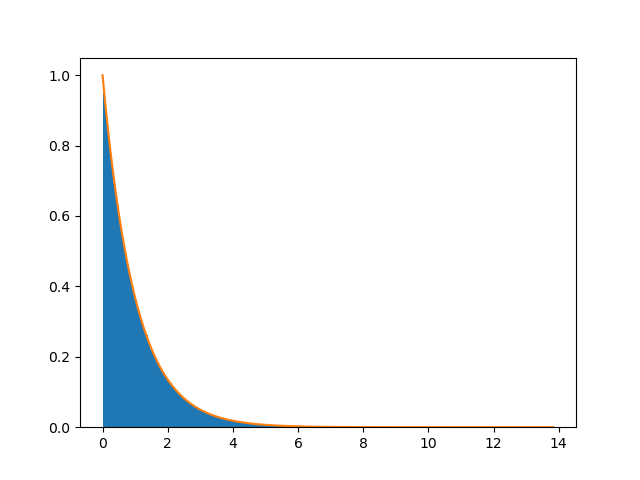
\includegraphics{2-3plot.png}
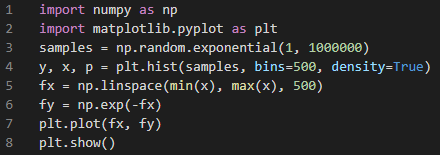
\includegraphics{2-3code.png}
\end{center}

%% Q3
\section{Optimal hedge ratio}
Assume that I own x shares of stock B, variance of total stock is
\[V(A+xB) = V(A) + x^2V(B) + 2xCov(A, B) = \sigma_A^2 + x^2\sigma_B^2 + 2x\sigma_A\sigma_B\rho\]
To minimize variance of total stock,
\[\frac{dV}{dx} = 2x\sigma_B^2 + 2\sigma_A\sigma_B\rho = 0\]
\[\Rightarrow x = -\frac{\sigma_A\rho}{\sigma_B}\]
Therefore, the number of share I have to sell n is
\[\bigg\{
\begin{tabular}{l r}
$n = x$ & $(\rho > 0)$ \\
$n = x + \frac{\sigma_A\rho}{\sigma_B}$ & $(\rho \leq 0)$
\end{tabular}\]

%% Q4
\section{Eigenvalues}

\[X = 
\begin{pmatrix}
1 & c & \cdots & c \\
c & 1 & \cdots & c \\
\cdots & \cdots & \cdots & \cdots \\
c & c & \cdots & 1
\end{pmatrix} = 
\begin{pmatrix}
c & c & \cdots & c \\
c & c & \cdots & c \\
\cdots & \cdots & \cdots & \cdots \\
c & c & \cdots & c
\end{pmatrix} +
\begin{pmatrix}
1-c & 0 & \cdots & 0 \\
0 & 1-c & \cdots & 0 \\
\cdots & \cdots & \cdots & \cdots \\
0 & 0 & \cdots & 1-c
\end{pmatrix} = C + (1-c)I\]
\[Rank(C) = 1 \Rightarrow dim(N(C)) = p-1\]
$ X-\lambda I = C$, so there are p-1 eigenvalues $\lambda_i = 1-c$.\\
Since $Tr(X) = p$, the last  eigenvalue $\lambda_p = p - (1-c)(p-1) = 1 + (p-1)c$, which have eigenvector $x_p = (1, 1, \cdots , 1)^T$

%% Q5
\section{Multivariate normal}

\subsection {}

$\Sigma$ is symmetric, so it can be decomposed to $\Sigma = QDQ^T = SS^T (S = QD^{\frac{1}{2}})$.\\
Let $X = SZ + \mu$,
\[E(X) = \mu + SE(Z) = \mu\]
\[V(X) = E((X-\mu)(X-\mu)^T) = E(SZZ^TS^T) = SE(ZZ^T)S^T = SIS^T = SS^T = \Sigma\]
Therefore, $X \sim N(\mu, \Sigma)$
\subsection {}
\begin{center}
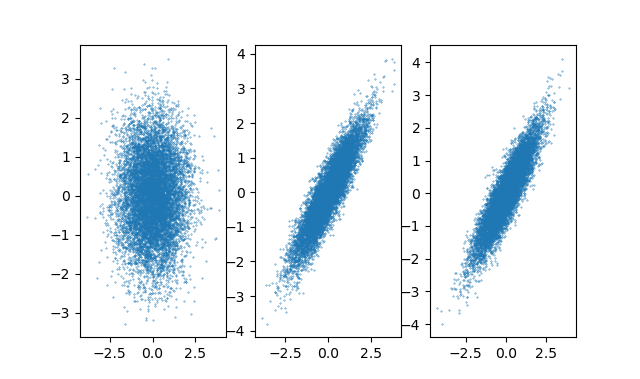
\includegraphics{5-2plot.png}
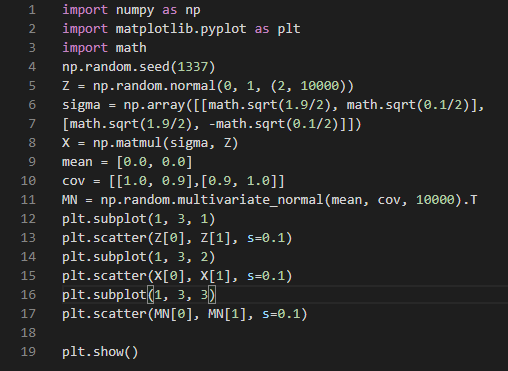
\includegraphics{5-2code.png}
\end{center}
%% Q6
\section{Optimization with positivity constraints}
Let $x_i$ = i-th element of vector $x$ and $v = x - x^*$. For $C = R_+^n$, $v$ that minimize $\nabla f(x^*)^Tv$ is
\[v_i = \bigg\{
\begin{tabular}{l r}
$-\nabla f(x^*)_i$ & $(x_i^* \neq 0)$ \\
$Max(-\nabla f(x^*)_i, 0)$ & $(x_i^* = 0)$
\end{tabular}\]
Therefore, simplified local minimum solution $x^*$ is
\[\bigg\{
\begin{tabular}{l r}
$\nabla f(x^*)_i = 0$ & $(x_i^* \neq 0)$ \\
$\nabla f(x^*)_i \geq 0$ & $(x_i^* = 0)$
\end{tabular}\]


\end{document}
